\documentclass[10pt,draftclsnofoot,onecolumn]{IEEEtran}

\usepackage{setspace}
\usepackage{caption}

% *** GRAPHICS RELATED PACKAGES ***
\ifCLASSINFOpdf
  \usepackage[pdftex]{graphicx}
  % declare the path(s) where your graphic files are
  \graphicspath{images/}
  % and their extensions so you won't have to specify these with
  % every instance of \includegraphics
  \DeclareGraphicsExtensions{.pdf,.jpeg,.png}
\else
\fi

% @TODO:
%   - go through and check that writing is in correct tense
%   - update screenshots
%   - add content to sections where relevant

% correct bad hyphenation here
\hyphenation{op-tical net-works semi-conduc-tor}

\begin{document}
\pagenumbering{gobble}
\singlespacing
\title{Spatial Visualization\\ of Biodiversity}

\author{Ty~Skelton,
        Jasper~LaFortune,
        and~Alec~Shields}% <-this % stops a space

% The paper headers
\markboth{CS 461}%
{Spring 2016}

% make the title area
\maketitle

% As a general rule, do not put math, special symbols or citations
% in the abstract or keywords.
\begin{abstract} % @NOTE: JASPER
The Department of Integrative Biology at Oregon State has collected a large sample of biodiversity data from various sites in the Southwest United States.
Handling this data in its raw form requires certain technical knowledge of databases, as well as a bit of patience.
This presents a problem for biodiversity researchers and Department of Defense land managers, who need to be able to understand and make decisions about this data easily.
Our team addressed this problem by creating a web interface for spatially visualizing this data.
We enabled users to easily display useful graphs and maps about areas and species of interest, putting the information they care about most at their fingertips.

The Department of Defense made an investment in collecting all these samples so that it could better manage its land.
However, extracting meaning from that information is challenging for land managers and researchers alike.
Any good solution to this problem would allow users to easily access the information that is important to them.
Our solution provides an interface that allows users to select information of interest and see it in map and graph form.
Passerby at Expo will be invited to interact with our system and discover meaningful biodiversity patterns for themselves.
Oregon State biodiversity researchers have indicated that our product meets their needs.

\end{abstract}
\IEEEpeerreviewmaketitle

\newpage
\pagenumbering{arabic}

\section{Project Purposes and Goals} % @NOTE: JASPER
This project aids researchers and land managers in drawing meaningful conclusions from a large set of insect biodiversity data.
The Department of Defense funded researchers to collect insect samples from many sites across the American Southwest over five years.
The resulting dataset is too cumbersome to make sense of in raw form, especially for land managers with little formal knowledge of database operations.
Our goal was to create a visualization system that allows these parties to select information of interest, display it on a map, and show useful graphs about it.

These requirements led us to a design comprised of three views.
The Filter View allows users to select which data will be displayed by date, season, species, or location, as shown in Figure~\ref{fig:overall_filter}.
The Map View shows the locations of the selected samples, as shown in Figure~\ref{fig:default_map}.
The Graph View shows graphs of the data selected in the Filter View broken down by location, taxa, and time, as shown in Figure~\ref{fig:graph_view}.


\section{Progress}

\subsection{Base Website Setup} % @NOTE: TY
When we were doing our technology review in preparation for writing our design document, we decided on using Django for our web framework, Apache for our web server, Git for our version control system, MySQL for our database, Bootstrap for our front end framework, and c3/arcGIS for our graphing/map views.
We have since organized and set up our back-end web framework correctly for our web app.
Since Django ships its beginning web structure in a very minimalistic state, (i.e. their templates, views, and models all in just one file with no app structure) We had to modularize those components into their own directories and files.
It wasn’t a long and arduous process, but it did take a bit of time learning how to go about doing that since we were all new to using Django.

Our web server configuration for development is now completely configured and deployed for off-campus access.
When we were still in development, we were making all of our features on our local machines.
We went through the process of deployment and have gone through the proper channels for gaining access to a remote server that we will put our web tool on.
Apache combined with mod\_wsgi.py were required for deploying our site statically on our remote server.
The only real challenge with getting Apache up and running was installing one dependency called mod\_wsgi.py which is required for Apache to serve Django content to the web, even on localhost.

Tracking our progress in development has been simple with Github.
We use the branching feature for each of us to introduce new features to our project.
Since each of us is in charge of one view (functionality) branching that is very easy and we still use it for making core changes to the framework.
We also track new features and issues with Git’s issue tracker and assign them all to milestones so we can properly prioritize changes by whether or not they’re in the coming release.

We all have some amount of experience interacting with MySQL, whether it be from our database class we took in pre-pro school or in the work force. That made converting our sponsor’s access database to MySQL much easier than it could’ve been, but it still was very challenging.
We have our system tied to the database perfectly and we are rendering data from it on our web page in different sections for a proof of concept.

Our front end framework we chose to implement was Bootstrap.
Bootstrap is a very well defined CSS/HTML framework and has seen use all kinds of applications, whatever the scale.

\subsection{Main Layout} % @NOTE: TY
As dictated in the design document, the main layout of the index page of our app is split into three sections.
Each section has been individually developed by each member of the team.
The top right view has an interactive map in a container.
In the top left there is a panel for filtering the data that is supplied to the other two views.
It has drop downs and date filters for better narrowing a field of data to fit what the user is looking for.
Finally, the index’s bottom container has a side-scrolling graph view that provides useful metrics on what the data consists of.
Each contained view has its own template that is embedded in a primary main template in an effort to keep the main template clean and organized.

\begin{figure}[h]
\centering
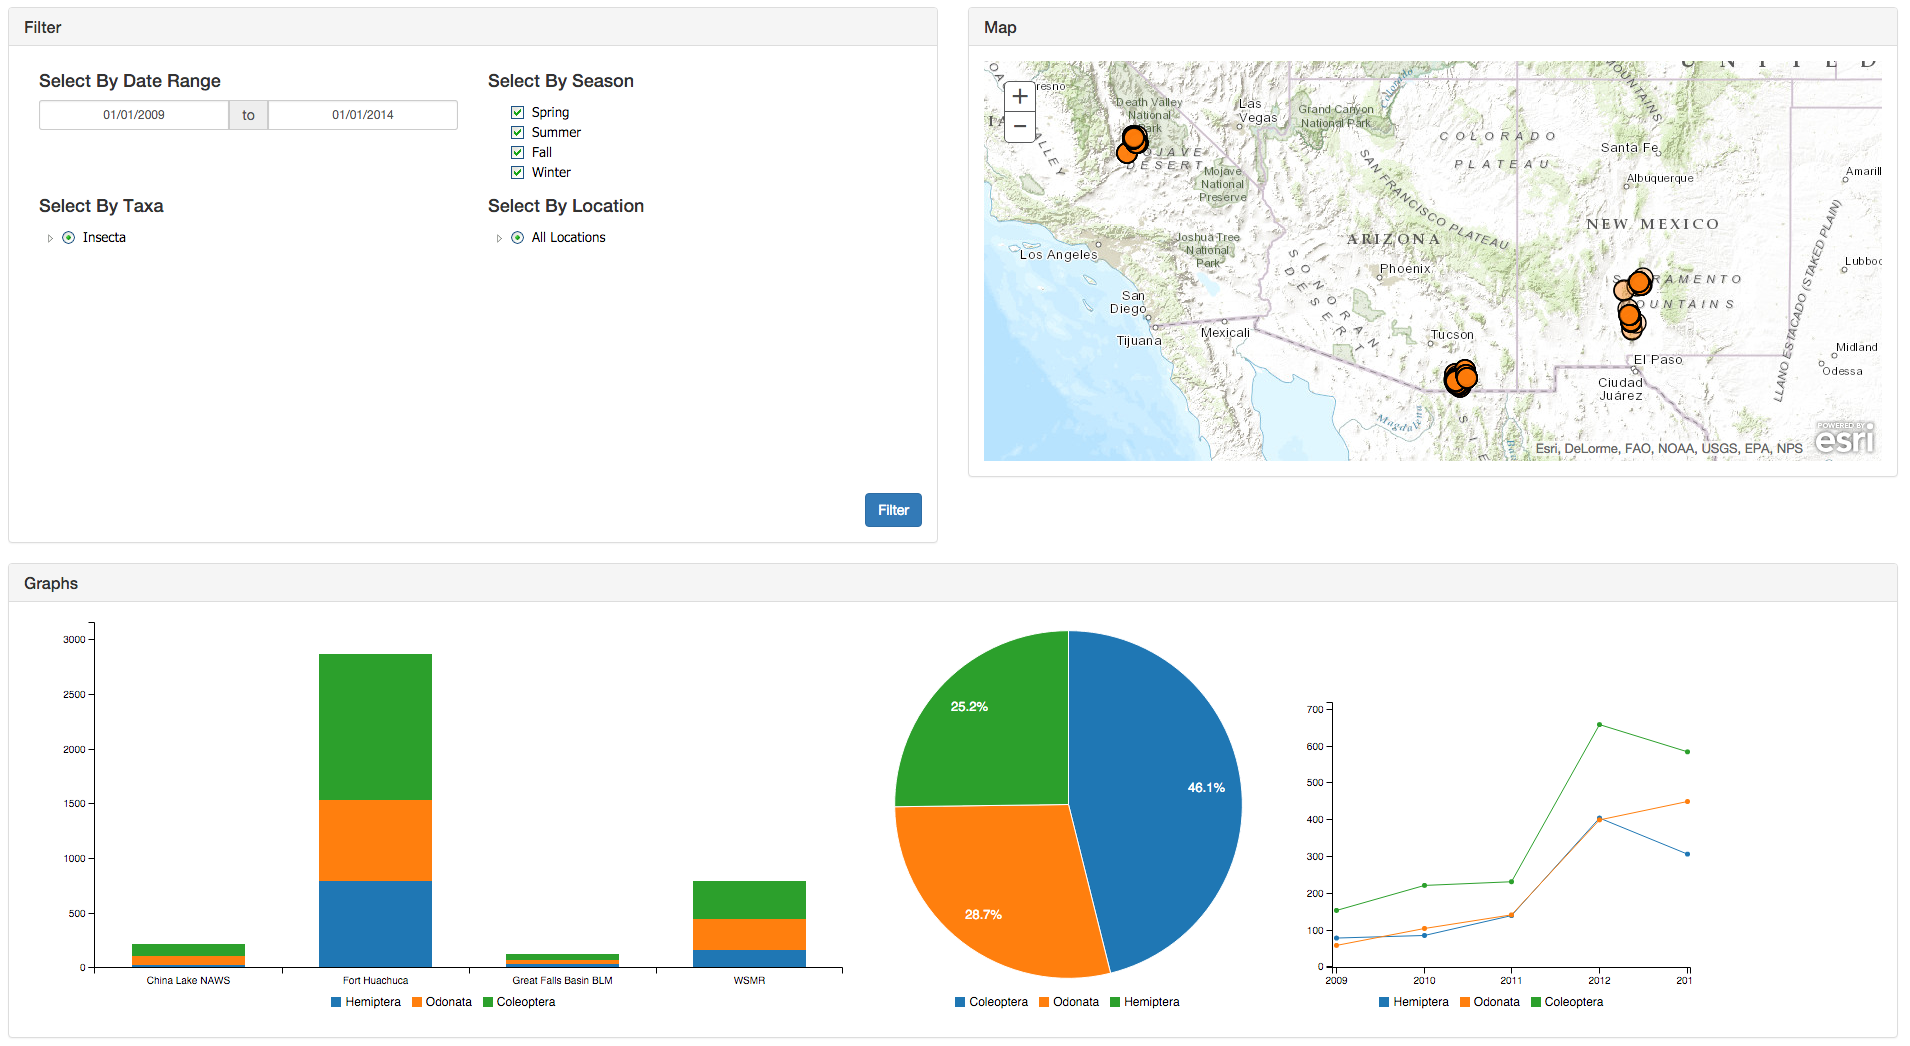
\includegraphics[width=0.75\textwidth]{images/main_layout.png}
\captionsetup{justification=centering}
\caption{
  Overall site layout view.
  upper left: filter view, upper right: map view, bottom: graph view.
}
\label{fig:layout}
\end{figure}

The main challenge with developing our single page web-app was providing data to the various tools we’re making use of in our different containers.
We have written models that map objects to database entries and allow us to provide serialized data to our templates.

\subsection{Filter View} % @NOTE: JASPER

The Filter View allows users to select information of interest by date, season, biological taxonomy, or site.
Selections made in the Filter View affect what is shown in the Map and Graph Views.
When the Filter View first loads, the user sees the pane shown in Figure~\ref{fig:overall_filter}.
By default, all data are selected.
The Date Range Filter begins populated with dates that capture the full range of data collection.
The Season Filter begins with all four seasons selected.
The Taxa Filter and the Site Filter begin fully collapsed, with the highest level selected.

\begin{figure}[h]
\centering
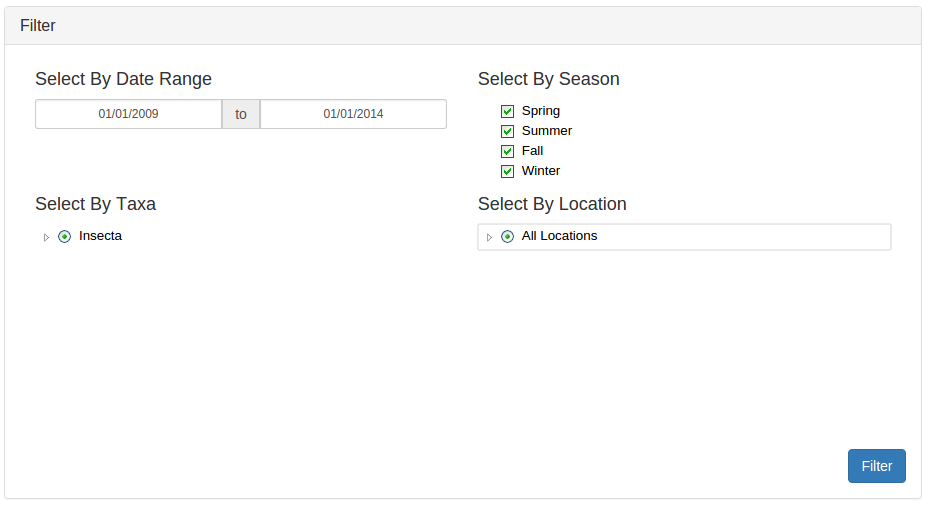
\includegraphics[width=0.75\textwidth]{images/overall_filter.png}
\captionsetup{justification=centering}
\caption{
  The Filter view contains four tiled filters, Date, Season, Taxa, and Location.
  By default, all data are selected and all children collapsed.
}
\label{fig:overall_filter}
\end{figure}

When the user makes selections in the Filter View, the Filter button changes color, as demonstrated in Figure~\ref{fig:date_filter}.
Clicking on the Filter button applies the selections made in the Filter View to the other two views.
Selections made in the Filter View persist on submission, so that the user can make selections serially.

The Date Filter allows users to view data from between a range of dates.
Clicking on either date field opens up a date range picker, shown in Figure~\ref{fig:date_filter}.
Users can also type in the date manually.
This causes the Graph View to only graph data collected between these two dates.
The Season Filter allows users to view data collected during certain seasons across all years.

\begin{figure}[h]
\centering
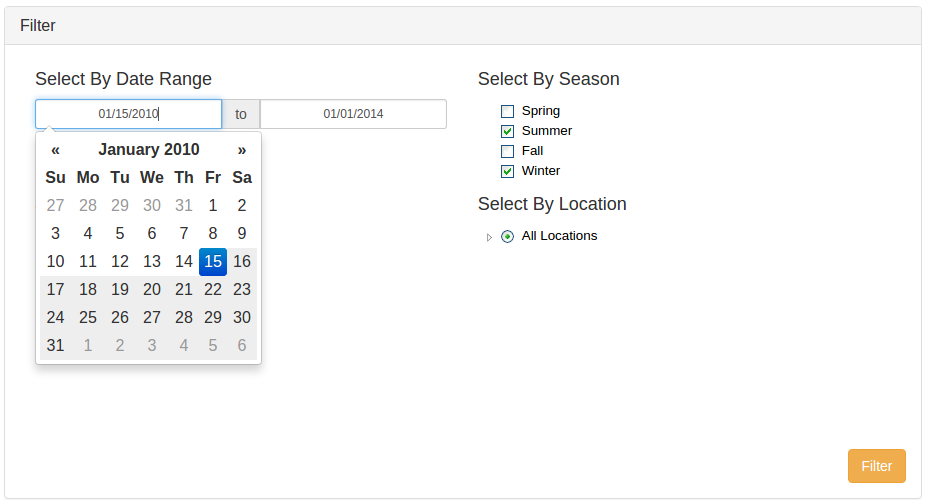
\includegraphics[width=0.75\textwidth]{images/date_filter.png}
\label{fig:date_filter}
\captionsetup{justification=centering}
\caption{
  When selections are made in the Filter View, the Filter Button changes color to indicate that submission is necessary.
  The Date Filter includes a date range picker.
}
\end{figure}

The Taxa Filter, shown in Figure~\ref{fig:taxa_filter}, allows users to select orders, families, genus, and species of interest hierarchically.
Users can select a radio button at any level in the hierarchy.
Selecting a parent node in the Taxa Filter supplies all the data from its children and none of the data from its siblings to the Graph View.
The Site Filter, shown in Figure~\ref{fig:location_filter}, allows users to select bases, drainages, sites, and samples of interest hierarchically.
Selecting a parent node in the Site Filter supplies all the data from its children and none of the data from its siblings to the Graph and Map Views.
Users can click on the triangle next to each parent to toggle whether its children are collapsed or expanded.
Expanding or collapsing children simply determines whether or not they show on screen, and does not affect selection.

\begin{figure}[h]
\centering
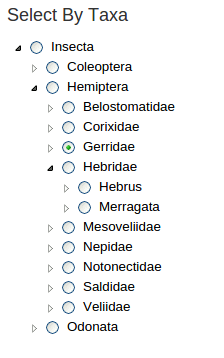
\includegraphics[width=0.25\textwidth]{images/taxa_filter.png}
\captionsetup{justification=centering}
\caption{
  The Taxa Filter allows the user to select an arbitrary level of biological taxonomy and all its children.
  For example, selecting the family Gerridae in the order Hemiptera selects all genuses and species in the Gerridae family.
  Because the input is a radio button, the user cannot simultaneously select siblings.
}
\label{fig:taxa_filter}
\end{figure}

\begin{figure}[h]
\centering
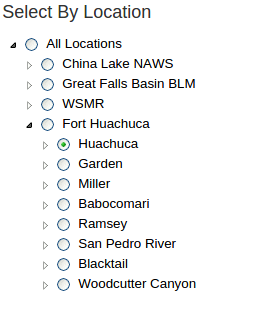
\includegraphics[width=0.25\textwidth]{images/location_filter.png}
\captionsetup{justification=centering}
\caption{
  The Location Filter allows the user to select an arbitrary location and all its children.
  For example, selecting the Huachuca drainage at the Fort Huachuca Base selects all sites in that drainage and all samples in those sites.
  Because the input is a radio button, the user cannot simultaneously select siblings.
}
\label{fig:location_filter}
\end{figure}

Jasper was assigned to developing the Filter View.
The main obstacle he faced was not any of the filters themselves, but rather the learning curve for the development workflow.
His experience using git for collaborative projects was limited, so on multiple occasions he called for help from the others.
His experience with web development was also limited, so tasks such as setting up a server required assistance.

When it came to writing code, the Filter View presented two main challenges.
The first was extracting meaningful information from the data posted by the filters.
To do this, we created a Filter Helper class that populates a dictionary with all the relevant fields for refining queries.
The second major challenge was making filter selections persistent.
To do this, we had to embed code in our HTML template to populate the fields from the data in the Filter Helper dictionary.
As such, data flows from the input forms in the Filter View, to the Filter Helper dictionary, back to the input forms.

\subsection{Map View} % @NOTE: ALEC

The map view changed quite a bit in its purpose throughout the development of our project.
In the brainstorming phase of our project we imagined it might be a kind of heat map of biodiversity in different areas.
We learned early on that this wouldn't be the purpose of the map view as it was to imprecise a way to compare data.
In addition, our data was coming from various collected points along rivers, which wouldn't make sense to make a continuous mesh across a map.
So we abandoned that idea early on in favor of comparing data using graphs based on the selected data.
Our next idea for the map view was to use it for selection instead.
We could select individual points or many points by drawing boxes over them.
However, we found that this was redundant as we were already using the filter view as a much more precise way of selecting the data to compare.
Using both would have been needlessly complicated and the points are so close together on the map that it wouldn't have worked well anyway.
After talking about these issues with the map with our client, we arrived at our final version of the map view, shown in Figure~\ref{fig:default_map}.

\begin{figure}[h]
	\centering
	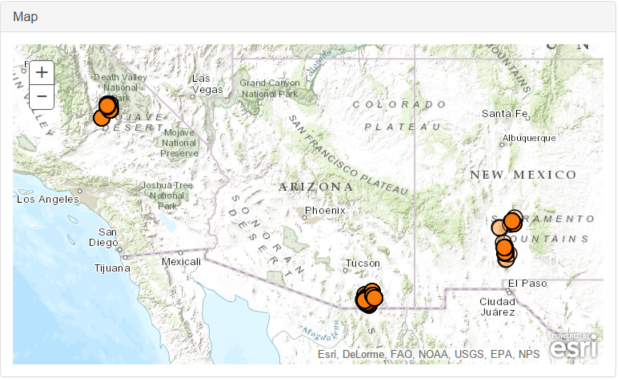
\includegraphics[width=0.50\textwidth]{images/default_map.png}
	\captionsetup{justification=centering}
	\caption{
		The default map view.
		This shows all the samples that were taken by the research team. The more opaque an area is, the more samples were taken there.
	}
	\label{fig:default_map}
\end{figure}

The purpose of this final map is to show the location and relative density of samples.
It plots every valid sample on the map as its own point.
These points are semi-transparent so that you can tell how dense the sampling in an area is based on how opaque that area is.
It is affected by the location and date filters, which ends up showing you where the data is coming from and where it is localized.
Every time the map is filtered it zooms to fit only the selected points which can be seen if Figure~\ref{fig:filtered_map}.
The map turned out a lot different than we first thought it to be, but it important in giving context to the data that is being viewed.

\begin{figure}[h]
	\centering
	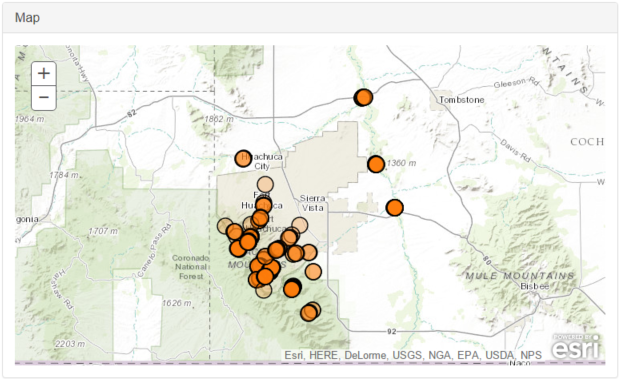
\includegraphics[width=0.70\textwidth]{images/filtered_map.png}
	\captionsetup{justification=centering}
	\caption{
		A filtered map view.
		This shows all the samples that are part of Fort Huachuca. It also zoom the map to cover just those points.
	}
	\label{fig:filtered_map}
\end{figure}

There where several major issues we ran into when working on the map view.
The first was the issue of UTM coordinates.
The data we had been given was in UTM coordinates which don't translate very well to the standard latitude and longitude coordinates.
Unfortunately, ArcGis doesn't work with UTM coordinates so we needed to make this conversion anyway.
To do that, we simply used a python script to calculate the coordinates for each sample and store the answer in new fields in the database.

The more difficult problem we had with the map was that several of the samples had bad coordinates.
In fact, many of the samples didn't have coordinates at all, or were missing a part of the UTM coordinate system.
This was a non-issue, as we could simply not display these coordinates.
However, we had several samples where the coordinates were input incorrectly, which caused them to show up in Mexico or the Pacific ocean.
These were more troublesome as they both misrepresented the data, and caused a vital feature of the map to work improperly.
Specifically, it caused the code that automatically fits the map to the current points to zoom out so far that you couldn't even see the map.
As you can imagine, this was a bit difficult to debug at first as we couldn't even seen the points that were causing the issue.
First, we looked at all the samples sorted by coordinates and hid the outliers.
This dealt with the points that showed up in the wrong areas, but there was still a point that was causing the weird zoom out bug.
To solve the issue, we made use of the filtering feature of our application.
We rendered different groups of points until we broke the map, then looked at each group within that group until we broke the map, and so on.
Eventually we had narrowed it down to the point that was causing the problem.
Then, we simply hid that point and the zooming feature of the map worked perfectly fine.

The map component of the project probably changed the most throughout development.
At first we envisioned it as a way to display biodiversity, then as a way to select our desired data.
We ended on using it as a way to give context to the data we are looking at, as well as displaying sample location and density.
While it changed a lot, we found a good way to make it useful to those using our application.

\subsection{Graph View} % @NOTE: TY
The graph view portion of our web tool is production-level ready.
We have fully developed charts deployed that render dynamically-loaded data based off of filter input.
Our graphs pull in data dynamically from the database and are then filtered down by the filter form variables.
Our currency for the graph data-points is number of unique species observed (except for the line chart which includes sampling rates).
The x-values are dynamically set to the sub-locations relative to the location level set in the filter field.

We currently have all three graphs in place that our client requested.
We are able to customize every aspect of them in regards to color, spacing, font, layout, etc.
An example of what the graph-portion looks like is shown in Figure~\ref{fig:graph_view}.
When the page is resized to be smaller, the graph window view will display a horizontal scroll bar so that the user can still see the metrics they’re interested in without having to make them too small to see.

\begin{figure}[h]
\centering
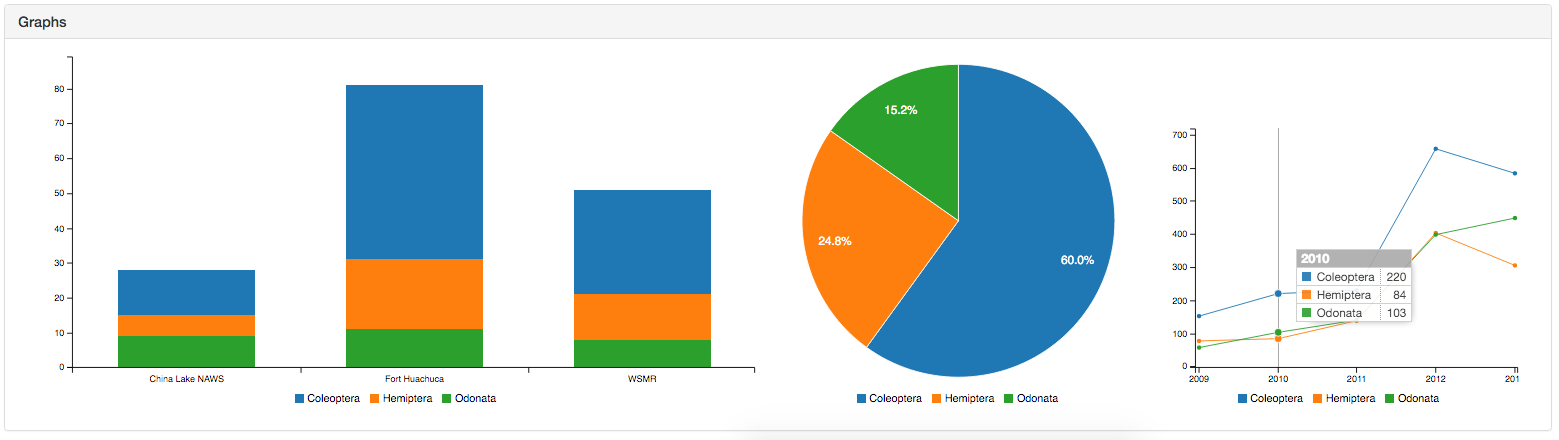
\includegraphics[width=0.75\textwidth]{images/graph_view.png}
\captionsetup{justification=centering}
\caption{
  The overall graph view.
  Displays dynamically generated charts on every page load and filter submission.
}
\label{fig:graph_view}
\end{figure}

The three different graphs that we were successfully able to pull data into and render meaningful statistics in were the stacked bar chat, pie chart, and line chart.
The stacked bar chart is showing the number of unique taxa within a certain taxonomic level at each location.
The pie chart is showing the distribution of unique taxa overall for all locations within the scope selected by the user.
Finally, the line chart is showing the number of unique taxa observed across all locations over time (years).

After the filter view submits a POST request to the index controller and figures out the parameters of interest (described in the filter section) an object with the necessary information is passed to the graph view.
Since the currency for the graph view is unique taxa observed, all the database queries and data massaging takes place in the subsample model.
After a particular graph retrieves the filter object it passes a generic query and refines it based on what the user is interested in.
Django uses lazy loading, meaning the query object is never processed until the code tries to parse it.
After the model gets the necessary information it has to format the two dimensional array in a very peculiar fashion for our graphing library to handle it (C3.js).
After it's formatted correctly, the model returns the array of arrays to the view, which stores it in the data object that is embedded in the view.
C3.js is loaded in the template as well, so we just embed the data object using Django's templating tools so it's parsed on load after all the dependencies.

\begin{figure}[h]
\centering
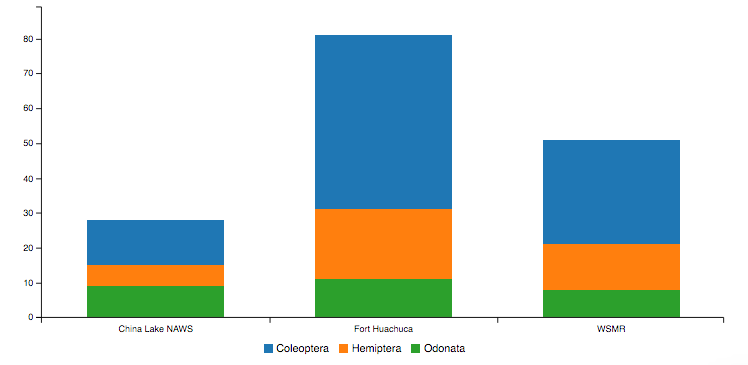
\includegraphics[width=0.70\textwidth]{images/bar_chart.png}
\captionsetup{justification=centering}
\caption{
  Stacked bar chart showing counts of unique taxa observed within a specified taxonomic level across varying locations.
}
\label{fig:bar_chart}
\end{figure}

The graph in Figure~\ref{fig:bar_chart_collapsed} displays a functionality in c3 that is really useful and is one of the primary reasons that we chose c3 as our graphing library for development.
If the user is to click (or touch on a touchpad) the label for a particular dataset within a graph, then the graph will hide that dataset and focus on only the remaining.
This is a very important functionality, because when taking biodiversity readings there could be an under-represented species or genus that only shares a small percentage of the dataset.
There could even be multiple that are dominated by one large collection.
If the user wants to ‘zoom in’ on those particular small readings, they could just hide the dominating dataset by clicking its label.

\begin{figure}[h]
\centering
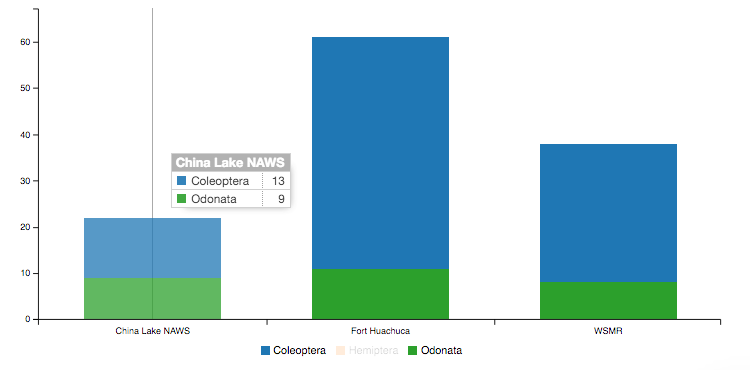
\includegraphics[width=0.70\textwidth]{images/bar_chart_collapsed.png}
\captionsetup{justification=centering}
\caption{
  An example of how the labels can be clicked to hide certain data displayed from view so the user can zero-in on a particular dataset.
}
\label{fig:bar_chart_collapsed}
\end{figure}

During development we encountered some varyingly-sized problems that slowed us down, but we were able to overcome them before production release.
The ability to supply data and render accurate graphs dynamically and accurately was our goal for the graph view come production release, but it took some hard work to get it to the point it's at.
None of us have used Django in the past and its ORM (object relational mapping) model structure, for constructing and querying objects from the database, was completely foreign to us.
Once we were able to learn how Django does it’s aggregate queries to the database it became a little bit more clear how to perform our queries, but it still proves to be challenging.
Early on after alpha release we were able to get all the static data supplied to the graphs replaced with dynamic data.
The end was in sight, but the ability to render dynamic x-values, labels, and y-values quickly became very difficult and it required a lot of clever problem solving to find a way to piggy-back data filtration logic in our filter helper models.
Once we were able to break through those barriers everything seemed to tone down in difficulty.
As we enter into the production-level phase of development we'll be doing much more polish and refinement than actual feature implementation, which is where we wanted to be.

\subsection{Database and Preparing Data} % @NOTE: ALEC

Creating the database and dealing with the raw data was a core component of the project that we anticipated would be one of the easiest, but gave us quite a few difficulties along the way.
Throughout development we went through several revisions in the design of our database as we grew to better understand the requirements of our project.
We also encountered quite a few more complications than we expected, mostly due to errors and inconsistencies in data entry.
These roadblocks set us back early on, as the database was essential for us to continue beta level development.
However, soon after our alpha release we ironed out the major issues with the database and quickly got our project up to the full-featured beta requirements.

The first step of preparing our database was creating a schema.
We initially used the schema we created for our design document, shown in Figure~\ref{fig:old_schema}.
This schema was more focused on breaking the data into smaller pieces that could be edited in application at a later date.
As we got further in design and discussed the data more with our client, we found that splitting the data up with way was unnecessary and only led to more work.
Another issue with the original schema was that the names of the different tables were slightly confusing to use in conversation.

\begin{figure}[h]
	\centering
	
\includegraphics[width=0.60\textwidth]{images/old_schema.png}
	\captionsetup{justification=centering}
	\caption{
		The first version of the schema.
		In this version the species specific information is in its own table, which we determined created unnecessary overhead.
	}
	\label{fig:old_schema}
\end{figure}

After much discussion and a meeting with our client, we arrived at our final version of our schema, shown in Figure~\ref{fig:new_schema}.
With this final version we renamed the sample groups to samples as they were the unit of a single collection of data.
We changed the sample in the original schema to subsample as they were all simply counts of a species in an overall sample.
The species data that was separated out in the initial version was merged into the subsample table as we had determined it did not justify the extra work.
Unlike the other tables, the sites table remained relatively unchanged.
During our meeting with our clients we also established which fields of the database were important and which were unnecessary.
At this point we had arrived at our final schema and could start the process of converting our raw data to be usable by our database and by extension our application.

\begin{figure}[h]
	\centering
	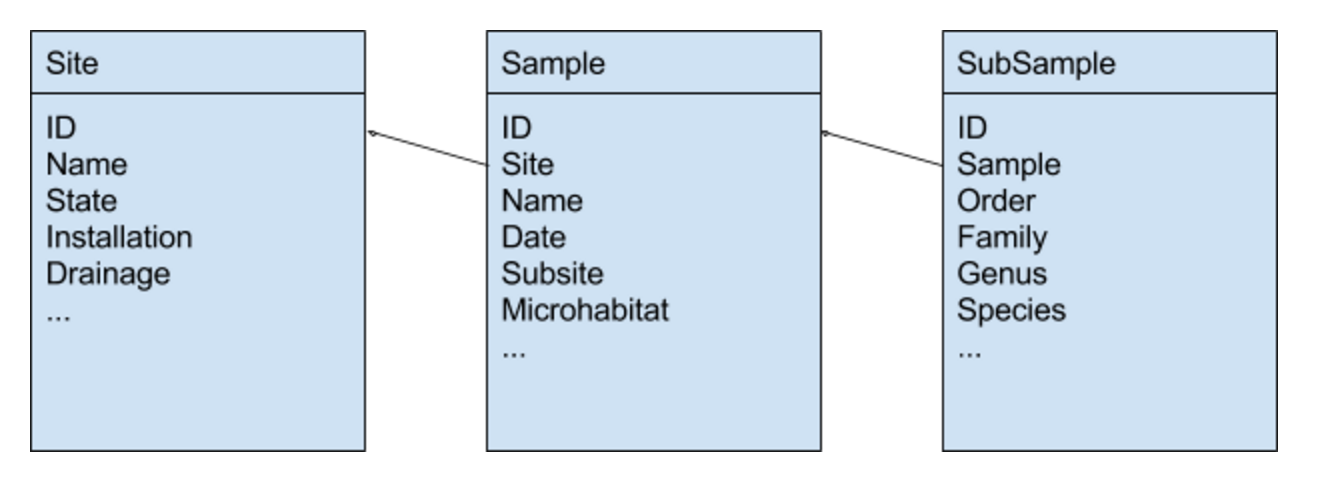
\includegraphics[width=0.70\textwidth]{images/new_schema.png}
	\captionsetup{justification=centering}
	\caption{
		The final version of the schema.
		This version renames sample group and sample to sample and subsample, respectively.
		It also merges the species table into the subsample table.
	}
	\label{fig:new_schema}
\end{figure}

Now that we had our schema we created a MySQL database that would hold our data, which proved very simple to accomplish.
Then came the hard part, converting the thousands of lines of manual data entry with no error-checking into a form usable by our system.
We were given the data in excel document format which wasn't ideal for our purposes.
Our first try to convert this document into a CSV that we could parse with a script.
This gave us trouble because some of the columns had commas in them.
Next we tried a CSV delimited on tabs, which also didn't work because some fields had tabs.
We did the same with semicolons but to no avail, as there were fields that had semicolons as well.
Eventually, we found that the problem column was the comments, were the data collectors wrote down various notes on the data.
We were told by our client that this column wasn't needed to we simple excluded that column and created a clean CSV with tabs as a delimiter.
With that we finally had our data in a form that we could parse with a script.

The next thing we did was create a python script to load our data into the database.
This script first started by loading the CSV into memory.
Then it iterated over each row and inserted the memory related to sites into the database.
It then did the same process again for both samples and subsamples.
The script was completely safe to run multiple times as it would check if an entry exists in the database before making an insertion.
At this point we had the data in the database, but would find that there were several issues that needed to be addressed before we could use all of it.

The first issue we encountered was with trying to make the data work with the map view.
The coordinates that were supplied in the data were in UTM coordinates, which were incompatible with the ArcGis mapping API that we were using.
While at first we thought this would be a simple conversion to latitude and longitude we found it was a very complex conversion between a flat system and a spherical system.
To remedy this we created two additional fields for latitude and longitude and created a python script that would populate these fields with the result of the complex calculation.
This made it so we wouldn't have to recalculate the latitude and longitude for every point every time we loaded the map.

The next issue we encountered was with there being errors in the coordinates provided.
Several points were being displayed on the map that were in Mexico or the Pacific ocean, two places where there was definitely so samples being taken.
After determining that these points were incorrect, we let our client know about them and decided to hide them from view as they were causing issues with the map's zooming feature.
A similar issue we had was with the inconsistency of the dates of samples.
Our client had requested a date filter that would show only data that was taken in a specified date range.
However, we found that the data was incredibly sparse and inconsistent when it came to the date it was taken.
Often times there was no date and sometimes the format of the date changed completely.
Our solution was to only filter based on the year that was a separate column that was much more consistent.
This wasn't an ideal solution and is definitely something we will bring up with our client next term.
After dealing with these issues, we had attained a beta level database that met our needs and requirements.

\end{document}
